\documentclass[tikz,border=3mm]{standalone}
% based on an answer by user http://tex.stackexchange.com/users/1952/ignasi
% on http://tex.stackexchange.com/questions/174317/creating-a-labeled-tetrahedron-with-tikzpicture
\begin{document}
\tikzset{>=latex}
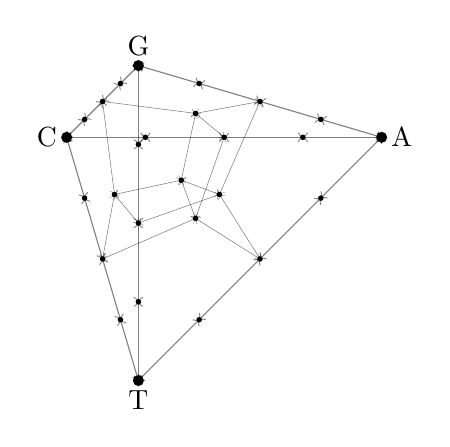
\begin{tikzpicture}[line join = round, line cap = round]
\pgfmathsetmacro{\xfactor}{1};
\pgfmathsetmacro{\yfactor}{1};
\pgfmathsetmacro{\zfactor}{1/sqrt(2)};
\coordinate [label=right:A] (A) at ( 2*\xfactor,  0*\yfactor, -2*\zfactor);
\coordinate [label=left:C]  (C) at (-2*\xfactor,  0*\yfactor, -2*\zfactor);
\coordinate [label=above:G] (G) at ( 0*\xfactor,  2*\yfactor,  2*\zfactor);
\coordinate [label=below:T] (T) at ( 0*\xfactor, -2*\yfactor,  2*\zfactor);

\coordinate [] (AACC) at  ( 0*\xfactor,  0*\yfactor, -2*\zfactor);
\coordinate [] (AAGG) at  ( 1*\xfactor,  1*\yfactor,  0*\zfactor);
\coordinate [] (AATT) at  ( 1*\xfactor, -1*\yfactor,  0*\zfactor);
\coordinate [] (CCGG) at  (-1*\xfactor,  1*\yfactor,  0*\zfactor);
\coordinate [] (CCTT) at  (-1*\xfactor, -1*\yfactor,  0*\zfactor);
\coordinate [] (GGTT) at  ( 0*\xfactor,  0*\yfactor, 2*\zfactor);

\coordinate [] (AAAC) at  ( 1*\xfactor,  0*\yfactor, -2*\zfactor);
\coordinate [] (ACCC) at  ( -1*\xfactor,  0*\yfactor, -2*\zfactor);
\coordinate [] (AAAG) at  ( 1.5*\xfactor,  0.5*\yfactor, -1*\zfactor);
\coordinate [] (AGGG) at  ( 0.5*\xfactor,  1.5*\yfactor, 1*\zfactor);
\coordinate [] (AAAT) at  ( 1.5*\xfactor, -0.5*\yfactor, -1*\zfactor);
\coordinate [] (ATTT) at  ( 0.5*\xfactor,  -1.5*\yfactor,  1*\zfactor);

\coordinate [] (CCCG) at  ( -1.5*\xfactor,  .5*\yfactor, -1*\zfactor);
\coordinate [] (CGGG) at  ( -0.5*\xfactor,  1.5*\yfactor, 1*\zfactor);
\coordinate [] (CCCT) at  ( -1.5*\xfactor,  -0.5*\yfactor, -1*\zfactor);
\coordinate [] (CTTT) at  ( -0.5*\xfactor,  -1.5*\yfactor, 1*\zfactor);
\coordinate [] (GGGT) at  ( 0*\xfactor, 1*\yfactor, 2*\zfactor);
\coordinate [] (GTTT) at  ( 0*\xfactor,  -1*\yfactor,  2*\zfactor);


\coordinate [] (ACG) at  ( 0*\xfactor,  0.6666667*\yfactor, -0.6666667*\zfactor);
\coordinate [] (ACT) at  ( 0*\xfactor,  -0.6666667*\yfactor, -0.6666667*\zfactor);
\coordinate [] (AGT) at  ( 0.6666667*\xfactor,  0*\yfactor, 0.6666667*\zfactor);
\coordinate [] (CGT) at  ( -0.6666667*\xfactor,  0*\yfactor, 0.6666667*\zfactor);
\coordinate [] (ACGT) at  ( 0*\xfactor,  0*\yfactor, 0*\zfactor);


\draw[<->, opacity=.5] (A) -- (AAAC);
\draw[<->, opacity=.5] (AAAC) -- (AACC);
\draw[<->, opacity=.5] (AACC) -- (ACCC);
\draw[<->, opacity=.5] (ACCC) -- (C);
\draw[<->, opacity=.5] (A) -- (AAAG);
\draw[<->, opacity=.5] (AAAG) -- (AAGG);
\draw[<->, opacity=.5] (AAGG) -- (AGGG);
\draw[<->, opacity=.5] (AGGG) -- (G);
\draw[<->, opacity=.5] (A) -- (AAAT);
\draw[<->, opacity=.5] (AAAT) -- (AATT);
\draw[<->, opacity=.5] (AATT) -- (ATTT);
\draw[<->, opacity=.5] (ATTT) -- (T);
\draw[<->, opacity=.5] (C) -- (CCCG);
\draw[<->, opacity=.5] (CCCG) -- (CCGG);
\draw[<->, opacity=.5] (CCGG) -- (CGGG);
\draw[<->, opacity=.5] (CGGG) -- (G);
\draw[<->, opacity=.5] (C) -- (CCCT);
\draw[<->, opacity=.5] (CCCT) -- (CCTT);
\draw[<->, opacity=.5] (CCTT) -- (CTTT);
\draw[<->, opacity=.5] (CTTT) -- (T);
\draw[<->, opacity=.5] (G) -- (GGGT);
\draw[<->, opacity=.5] (GGGT) -- (GGTT);
\draw[<->, opacity=.5] (GGTT) -- (GTTT);
\draw[<->, opacity=.5] (GTTT) -- (T);


\draw[<->, opacity=.5, very thin] (AACC) -- (ACG);
\draw[<->, opacity=.5, very thin] (AAGG) -- (ACG);
\draw[<->, opacity=.5, very thin] (CCGG) -- (ACG);

\draw[<->, opacity=.5, very thin] (AACC) -- (ACT);
\draw[<->, opacity=.5, very thin] (AATT) -- (ACT);
\draw[<->, opacity=.5, very thin] (CCTT) -- (ACT);

\draw[<->, opacity=.5, very thin] (AAGG) -- (AGT);
\draw[<->, opacity=.5, very thin] (AATT) -- (AGT);
\draw[<->, opacity=.5, very thin] (GGTT) -- (AGT);

\draw[<->, opacity=.5, very thin] (CCGG) -- (CGT);
\draw[<->, opacity=.5, very thin] (CCTT) -- (CGT);
\draw[<->, opacity=.5, very thin] (GGTT) -- (CGT);


\draw[<->, opacity=.5, very thin] (ACG) -- (ACGT);
\draw[<->, opacity=.5, very thin] (ACT) -- (ACGT);
\draw[<->, opacity=.5, very thin] (AGT) -- (ACGT);
\draw[<->, opacity=.5, very thin] (CGT) -- (ACGT);


\foreach \i in {ACGT}
    \fill [black] (\i) circle (1pt);

\foreach \i in {ACG, ACT, AGT, CGT}
    \fill [black] (\i) circle (1pt);

\foreach \i in {AACC,AAGG,AATT,CCGG,CCTT,GGTT,AAAC,ACCC,AAAG,AGGG,AAAT,ATTT,CCCG,CGGG,CCCT,CTTT,GGGT,GTTT}
    \fill [black] (\i) circle (1pt);
\foreach \i in {A,C,G,T}
    \fill [black] (\i) circle (2pt);

\end{tikzpicture}

\end{document}

% AXES
%\draw[->] (0,0) -- (3,0,0) node[right] {$x$};
%\draw[->] (0,0) -- (0,3,0) node[above] {$y$};
%\draw[->] (0,0) -- (0,0,3) node[below left] {$z$};
